\important{Artificial Intelligence Improvements  (December 18, 2024)}
\label{AI-Improvments (December 18, 2024)}
\chapterauthor{Ian Smith}
\info{Ian Smith}{AI Improvements}{December 18, 2024}
\section*{AI Training Progress Report }

\subsection*{Think Tank and Initial Observations}
During the team's scheduled practice time on December 17, 2024, the team met to conduct a brainstorming session focused on AI training. We determined that the AI is learning effectively enough to warrant serious exploration within the team; it is no longer considered a side project. However, the challenge now lies in designing an appropriate reward system for training.

\subsection*{Initial Training Setup}
We removed all distractions from the simulator, simplifying the environment so that the AI moves toward a single target point on the field. The initial reward structure at the start of the night was defined as:
\[
    r = dist_{t, a}^2
\]
This reward structure created a heat map that the network used to determine reward distribution. During the first training session, the robot learned to move toward the heat signature, but its performance was not highly accurate.

\subsection*{Refinements to the Reward Function}
To improve the AI's accuracy, we experimented with several adjustments to the reward function:
\begin{itemize}
    \item Removed the piecewise element to simplify the training process.
    \item Added a steady reward for capturing the object in the forward-facing camera.
    \item Widened the camera lens to broaden the field of view.
    \item Narrowed the camera lens to encourage precise targeting of the object.
\end{itemize}
Unfortunately, none of these modifications produced significant improvements.

\subsection*{Rejected Solutions}
Several other solutions were proposed but ultimately rejected due to feasibility concerns:
\begin{itemize}
    \item \textbf{Adding a secondary network to calculate weighted rewards:} This approach was dismissed due to the complexity and time required to develop an additional network and reward function.
    \item \textbf{Incorporating additional sensors:} This solution was deemed impractical, as the real-world application limits the ability to add more sensors to solve the problem.
\end{itemize}

\subsection*{Current Approach and Preliminary Results}
Our final attempt involved feeding the AI the difference in distance between the calculated optimal heading and the current heading. While we could not complete this approach during practice, we began implementing the following methodology:

\begin{figure}[H]
\centering
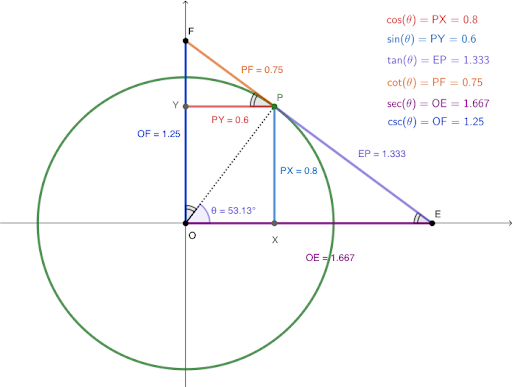
\includegraphics[width=0.5\textwidth]{images/Ian'sTrig.png}
\caption{Visualizing the Trigonometric Measurements with a Circle and a Tangent. \cite{anirdesh}}
\label{fig:anirdesh}
\end{figure}

To calculate the optimal heading, we used the coordinates of the robot ($O$) and the object ($P$) to form a right triangle. The first step was to calculate the hypotenuse $h$. While the Pythagorean theorem could be used ($h = \sqrt{a^2 + b^2}$), we demonstrated the process using length and angle relations:
\[
    h = \frac{o}{a}
\]

Next, we solved for the angle $\angle POX$. Let $A$ ($\angle PXO$) equal 90 degrees, $S_x$ be $P_x - O_x$, and $S_y$ be $P_y - O_y$. Using the law of sines, we determined the missing angle $\alpha$:
\[
    \frac{h}{\sin{90}} = \frac{S_y}{\sin{\alpha}}
\]
Rearranging the equation allowed us to isolate $\alpha$ for further calculations.

\section*{Conclusion and Next Steps}
The team has made significant progress in training the AI, moving from basic learning to more complex refinements of the reward structure. Despite challenges, we are optimistic that the current approach will yield better results in future practice sessions. Further experimentation and validation are required to ensure robust performance in real-world scenarios.
{"originatingScript":"m2","payload":{"guid":"bd5b3fe5-bcb6-4473-8dc3-8775bd7bbea10f21df","muid":"e85d44aa-714f-4310-b8c8-cfba21cef6ea7c9fc6","sid":"5c7e69f0-25ea-480f-ae0e-250fedf7bb4daad3dd"}}